%!TEX root = ../../dissertation.tex
%%%%%%%%%%%%%%%%%%%%%%%%%%%%%%%%%%%%%%%%%%%%%%%%%%%%%%%%%%%%%%%%%%%%%%%%%%%%%%%%
\chapter{Streaming in Mobile Networks}
\label{chap:mobilestreaming}


%%%%%%%%%%%%%%%%%%%%%%%%%%%%%%%%%%%%%%%%%%%%%%%%%%%%%%%%%%%%%%%%%%%%%%%%%%%%%%%%
\section{Introduction and Background}


%%%%%%%%%%%%%%%%%%%%%%%%%%%%%%%%%%%%%%%%%%%%%%%%%%%%%%%%%%%%%%%%%%%%%%%%%%%%%%%%
\section{Proposals}


%%
\section{Upcoming Protocols and Streaming Relationship}

\begin{itemize}
\item SPDY / HTTP/2.0 (multiplexing -> segmented streaming)
\item TCP changes (Fast Open, IW10, ...; any relationship to streaming? maybe faster)
\item Alternate Transport Protocols (DCCP\cite{rfc4340}, LEDBAT\cite{rfc6817}/$\mu$tp\cite{bt2010utp}, QUIC, SCTP, DTLS), HTTP/2.0 draft TODO
\end{itemize}


\begin{itemize}
\item Compensation mechanisms for reliable transport
\item Model and quality estimations for improvements to adaptive streaming
\item End-to-end encryption and Authentication mechanisms (e.g.IPSec, DNSSEC, CurveCP) %(Daniel J. Bernstein)
\item Modifications to and issues with TCP
 \begin{itemize}
 \item TCP buffer bloat
 \item Initial window size (IW10, ...)
 \item WebSockets as streaming transport \cite{w3c2011websockets} \cite{heise2011websockets}
 \item WebRTC
 \item Relevance of multicasting or similar techniques for streaming transport (real-time live vs. stored)
  
 \item
 \end{itemize}
 \end{itemize}


%%
\subsection{Influence of Layers}

Wired Internet access has a very narrow choice of protocols on the ISO/OSI Layers 1 and 2. The typical use-case consists of a Local Area Network using Ethernet which is then tunneled through or translated into one of several access technologies, e.g., DSL, DOCSIS, or PON. Applications often make assumptions that rely on the presence of these protocols and their specific characteristics.

However, Internet access today is similarly often achieved using mobile cellular networks. The latest standardized iteration of these is LTE and the accompanying EPS core network infrastructure \cite{olsson2009sae}. This is the first evolution of standards that completely removes the classical circuit switched domain making room for more radio frequency bandwidth to be used with the all-IP services achieving shared transmission capacities -- comparable to today's 802.11n WiFi -- albeit on much larger cell sizes of 1 to 30 kilometres. The EPS network (cf. Fig. fig:ltecore) acts as an intermediary between the radio access stations and the Internet enabling strong traffic control mechanisms as well as mobility anchored at the Serving Gateway (S-GW). Traffic is routed through the core by using tunneling over the S-GW and P-GW based on the traffic bearer concept defined either in the GTP or the PMIPv6 protocols. For every mobile device connected to the network there is one default and up to ten dedicated bearers carrying traffic filtered by pre-set QoS parameters. Control is enforced through a logically separate network control plane, that is also used to setup and tear down these bearers. Figure fig:ltestack displays the disparity between the Internet's protocol stack and that of an LTE network encapsulating all user traffic in additional protocol layers by the tunneling process.

Research work is ongoing how to best work with this complex network setup. It is expected, that with the rise of mobile access the core network comes under heavy traffic pressure with negative affects on the QoS of best-effort traffic. Endeavors are required to study the loaded network's behavior. Also very little work has gone into exploring the control plane characteristics of these networks, including their performance. A novel approach could also be, to make mobile device applications, e.g. video streaming players, aware of the core networks capabilities and allow the request of tunnels tailored to their specific QoS requirements resulting in a possible increase of perceived quality.

% influence of signaling plane and core network elements - scaling

The protocols used for the radio transmissions behave very differently when compared to Ethernet and assumptions made by higher layers may not hold any more. This can apply to, e.g., reliability, frame sizing and fragmenting, and latency amounting to undesired effects on higher-layer traffic. For example, loss in GSM and UMTS networks is often caught transparently on layer 2 and a retransmission is conducted. However, in the time the retransmission takes the transport layer may have already run into a timeout and re-requested the missing segment on its own, resulting in additional delay and a waste of bandwidth. This is especially detrimental for time-critical applications like video streaming, possibly resulting in buffer underruns and degraded quality. Transport and application layer mechanisms need to be able to understand this and cope with the effects. E.g., TCP retransmissions and congestion control could be adjusted in the course of understanding this.

Furthermore, traffic could be avoided during cell handover occurrences. This would require cross-layer cooperation and an awareness of the application when an handover is supposed to occur. The application then could schedule its traffic accordingly. Traffic falling into a handover is subject to especially high latency and loss because the mobile network acts as a mobility anchor which needs to internally reroute incoming traffic to the mobile device's new position. HTTP traffic is especially suited to this scheduling behavior because of its statelessness and consistence of small objects that can be requested and transferred independently.


%%
\subsection{Cross-Layer Mobility Hinting}
\label{c5:crosslayerhinting}

i.e. Mobility without network support

Why? Handovers mean very long application interruption, and redirecting tcp flows to the current base station isn't cheap either (also, induces \textbf{very} long latency)

\begin{itemize}
\item Tell Transport/Application the expected time till handover / time of uninterrupted service
\item Tell Transport/App expected connection parameters (latency, BW, ...)
\item Application selects DASH stream appropriate to parameters
\item Application reorders HTTP GETs so that large GETs are not interrupted
\item Application stops transfers when handover is about to occur
\item Layer 1/2 gives a list of possible handovers to Application
\item Application selects (better: suggests) handover which fits best and reorders accordingly
\end{itemize}

Advantages/Disadvantages?

Violation of Layering/encapsulation? No, only APIs get extended 

TOBECONTINUED

SmoothIT mechanisms; lower layer elements provide information to higher layers, overlays  \cite{oechsner2009pushing}


Network Unassisted/Independent Mobility / Mobility Prediction API: When will the next handover occur, how much delay and bandwidth do i currently have? Can i complete oustanding transfers or should i reschedule them? Or, e.g., should i request a lower quality fragment? // Requirements: Stateless short to midtermed ``Connections'', high granularity of data ``packets''
--> ``Mobility Awareness'' \cite{hummel2010mobilitaet} PMLAR (Predictive mobility and location-aware routing protocol in mobile ad hoc networks)





%%%%%%%%%%%%%%%%%%%%%%%%%%%%%%%%%%%%%%%%%%%%%%%%%%%%%%%%%%%%%%%%%%%%%%%%%%%%%%%%
\section{Investigations}


%%
\subsection{Streaming Mobile Adaptation}



%%
\subsection{Mobile Measurements with Additional Metadata}
\label{c5:sensorium}

SENSORIUM EXCURSION
CONTEXT: (active) measurements in mobile networks should make use of the device's current state and environment. i.e., read its sensor data and put measurements in context with it. Alternatively, use anonymized sensor data for new kinds of evaluations (can this device watch video at all at the current location?)
CONTEXT

Modern computing devices such as smartphones, laptops, and tablet computers are equipped with an increasing number of sensors: GPS, tilt, and acceleration meters quantify the physical position and orientation of the device; 3G, WiFi, and other  interfaces gather data on the availability and signal quality of wireless networks; temperature and ambient light sensors deliver additional insight into a user's work and home environments.

There exist problems for the practical viability of collection data though: Different devices and platforms such as Android and iOS use very different interfaces into their sensors; privacy is another issue hardly tackled on any platform other than in a crude binary (allow/deny access) way. Therefore, in this demo we introduce Sensorium, a generic sensor reading framework that funnels data from actual sensor drivers, implements fine-grained privacy control for the user, and provides generic outbound interfaces such as XML-RPC. We also show an application using it, O3GM, which visualizes mobile coverage data coming from Sensorium.

%Sensor interfaces differ -> difficult to do generic stuff with them
Sensorium can access all the information a device provides and makes them available to other applications. Up until now, it has been a challenging task for software developers (especially scientists and experimenters) to implement specialized sensor applications. This task is simplified by providing a generic framework for interfacing sensors. In our current implementation, available for Android, most of the typical sensors are already implemented. Since giving access to sensor data also exposes the user's privacy, the user can disable or set privacy levels for each sensor individually, and all sensor readings that would be shared are displayed. %Setting higher privacy levels reduces the amount of data a sensor shares. %E.g., location data accuracy could be rounded, or just hashes of data shared.
\\

O3GM\footnote{\url{http://homepage.univie.ac.at/albert.rafetseder/o3gm}} showcases the sensors framework. It comprises a web service displaying cellular access technology data points at their GPS locations collected by devices running Sensorium (see Figure~\ref{c5:fig:ogggm}). This solves a real-world problem: Currently, this kind of data is only available to mobile operators, which however  are hindered by commercial interests to make them publicly available -- at least in raw, unadorned form. Other projects such as OpenSignalMaps\footnote{\url{http://opensignal.com/}} and Sensorly\footnote{\url{http://www.sensorly.com/}}, as well as corporations like Google and Apple collect these data, but are very restrictive regarding usage by other parties. This is not true for O3GM: We make the data points collected available as Open Data under an open content license.

Obviously, other applications are possible. Since code and data are open-sourced, everyone can implement their great ideas, port Sensorium to other platforms or reimplement our interface there, etc.

\begin{figure}[htbp]
\centering
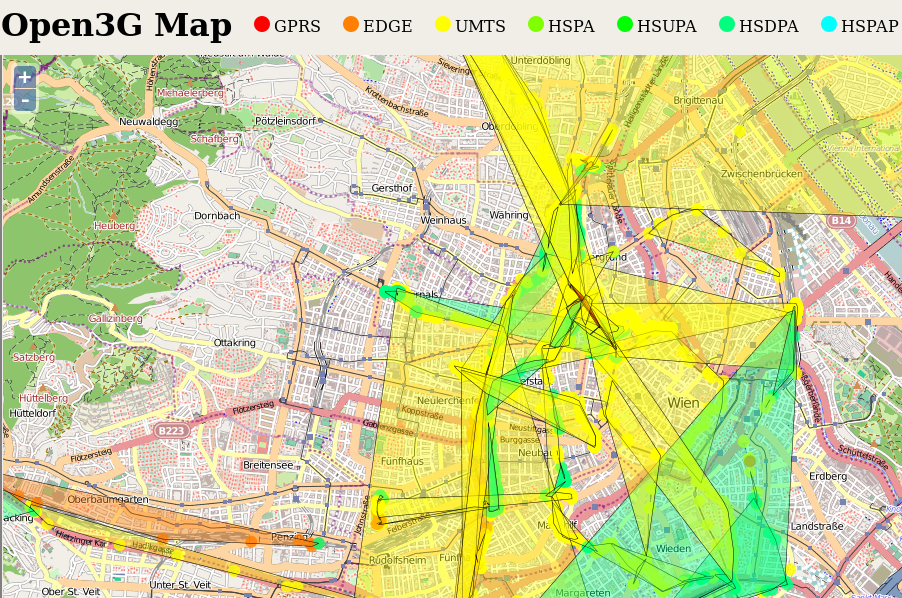
\includegraphics[width=.98\columnwidth]{images/map-cells.png}
\caption{\small The O3GM web page, displaying 3G coverage measurements extracted from Sensorium on top of OpenStreetMap.}
\label{c5:fig:ogggm}
\end{figure}

\subsubsection{Architecture}

Figure~\ref{c5:fig:architecture} overviews Sensorium's architecture components, and its interplay with the data collecting parts of O3GM. \textit{Sensor drivers} are implemented on top of the operating system taking care of reading sensor values from platform-specific interfaces and pushing them upwards into the \textit{registry}. Here, sensor data is timestamped and collected. On one side, data are prepared for local display, e.g. in a GUI or status widget. On the other side, a user-configurable \textit{privacy layer} might allow for full sensor access from above or reduce the precision of values (e.g. round GPS coordinates); it could salt and hash sensor values for improved privacy, or completely deny access to individual (or all) sensors. Finally, other applications running on the same device are free to connect to Sensorium's \textit{outbound interfaces} to register for sensor updates or poll data. Access from sources other than localhost is not allowed for obvious privacy reasons.

Due to the layered architecture, it is very simple for contributors to add their own implementations of layers or swap them out for their own altogether. Consider a scenario when a contributor wishes to include a sensor we do not yet provide a driver for. All that needs to be implemented is code interfacing the actual sensor, and the lightweight API into our sensor registry. Similarly, additional local display methods, privacy enhancements, and outbound interfaces might be implemented.

\begin{figure}[t!]
\centering
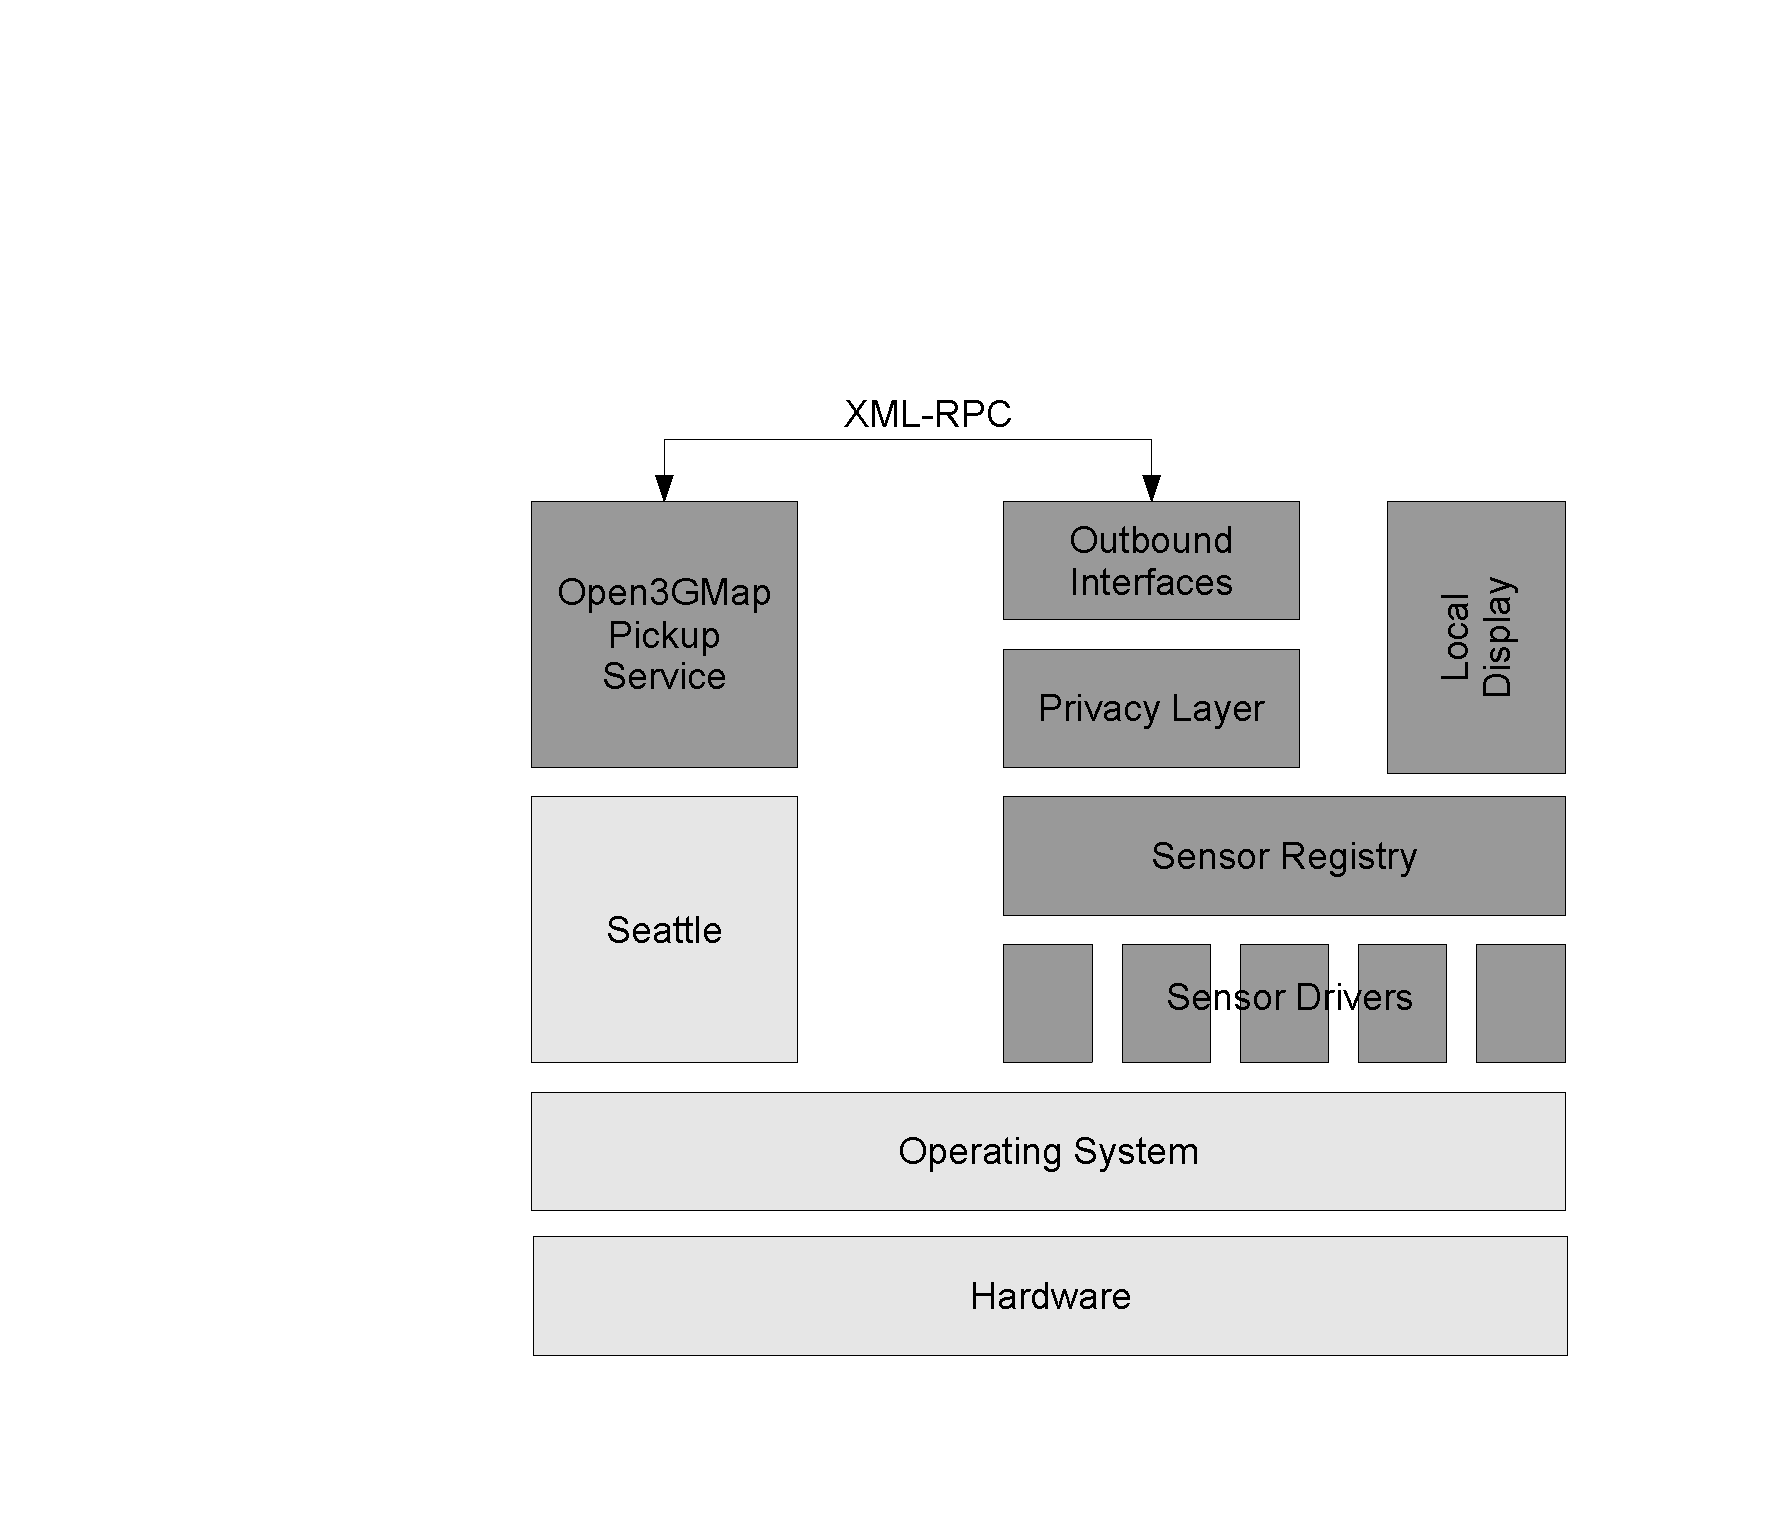
\includegraphics[width=0.85\columnwidth]{images/architecture.pdf}
\caption{\small Sensorium architecture with O3GM \textit{pickup}~and \textit{server}. Components described in this paper are shown dark gray.}
\label{c5:fig:architecture}
\end{figure}

\subsubsection{Implementation}

Our current implementation of Sensorium\footnote{\url{https://github.com/fmetzger/android-sensorium}} runs on the Android platform. To provide a unified interface for accessing the sensor data we incorporated an XML-RPC library\footnote{\url{https://code.google.com/p/android-xmlrpc/}} that listens for connections on localhost, meaning that only applications running on the same device can access it. The pickup code\footnote{\url{https://homepage.univie.ac.at/albert.rafetseder/o3gm_pickup.repy}} to collect sensor values runs on top of the renowned Seattle\footnote{\url{https://seattle.cs.washington.edu/}} platform, which is also available for Android, and allows us to remotely and securely access the collected data, and easily experiment with energy and cost efficient data upload/download strategies. The example application we implemented to make use of Sensorium, O3GM\footnote{\url{https://github.com/lukpueh/Open3GMap}}, is based on JavaScript and the OpenLayers\footnote{\url{http://openlayers.org/}} library. All of our code is dual-licensed under GPLv3 and the BSD license.

\begin{figure}[t!]
\centering
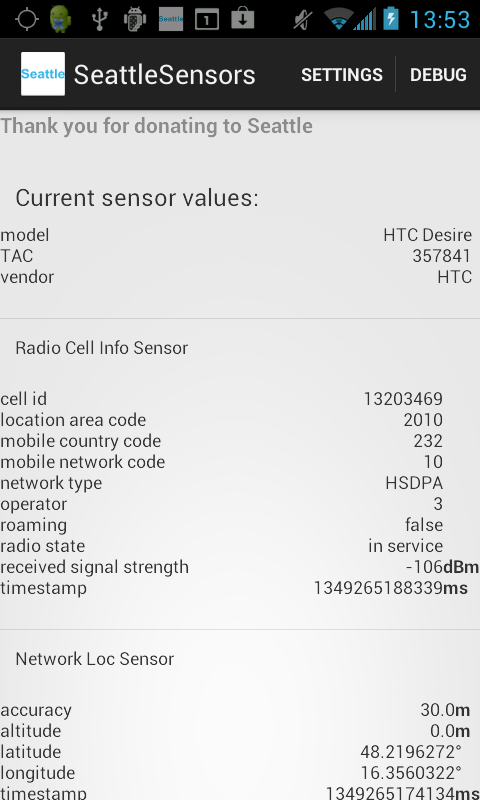
\includegraphics[width=0.45\columnwidth]{images/sesescreenshot.png}
\caption{\small Sensorium screenshot.}
\label{c5:fig:screenshot}
\end{figure}

Sensorium consists of a base registry service with a common interface which each sensor implementation can easily be plugged into. All values are also displayed for the user as seen in Figure~\ref{c5:fig:screenshot}. The privacy layer automatically anonymizes all gathered values before making them available through XML-RPC in accordance with the user's current privacy settings.

We currently provide sensor implementations for generic device information, e.g. device name and battery status; mobile radio data such as current access technology and cell information; location data provided by the mobile network and GPS; and  WiFi and Bluetooth information, including recent scan results.

Sensorium attempts to bring the sensing capabilities of current generation devices to a broader range of developers and experimenters. Directly using Sensorium, which is freely available from the Google Play store, or adopting the available source code gives everyone the chance to build projects like the mobile coverage Web service we presented.


%%%%%%%%%%%%%%%%%%%%%%%%%%%%%%%%%%%%%%%%%%%%%%%%%%%%%%%%%%%%%%%%%%%%%%%%%%%%%%%%
\subsection{Measurement Approaches}
\label{c5:mobilestreamingtestbed}

Different Approaches

\subsubsection{Simulating Streaming Traffic Characteristics in ns-3}

TODO: Implement a HTTP Streaming Traffic Generator ns-3 Application and a streaming receiver client application.
TODO: Use LENA to transport streams
TODO: Use Python
TODO: Maybe base it on http://code.google.com/p/tmix-ns3/ ?
TODO: Maybe use ON-OFF traffic generator with streaming specific patterns; cf. to http://www.nsnam.org/docs/release/3.17/doxygen/classns3\_1\_1\_on\_off\_application.html\#details


\subsubsection{Mobile Streaming Simulation/Emulation Hybrid Test Platform}

Use introduced streaming evaluation approaches in a mobile network environment

But do not want to use real network, as conditions are hard to manage and reproduce. Additionally, LTE still hard to come by.

Therefore, use an emulated network provided by the ns-3 network simulator. But transmit real traffic through it, i.e. use it as an emulator and bridges. \ref{fig:lte-testbed}

\begin{figure}
\centering
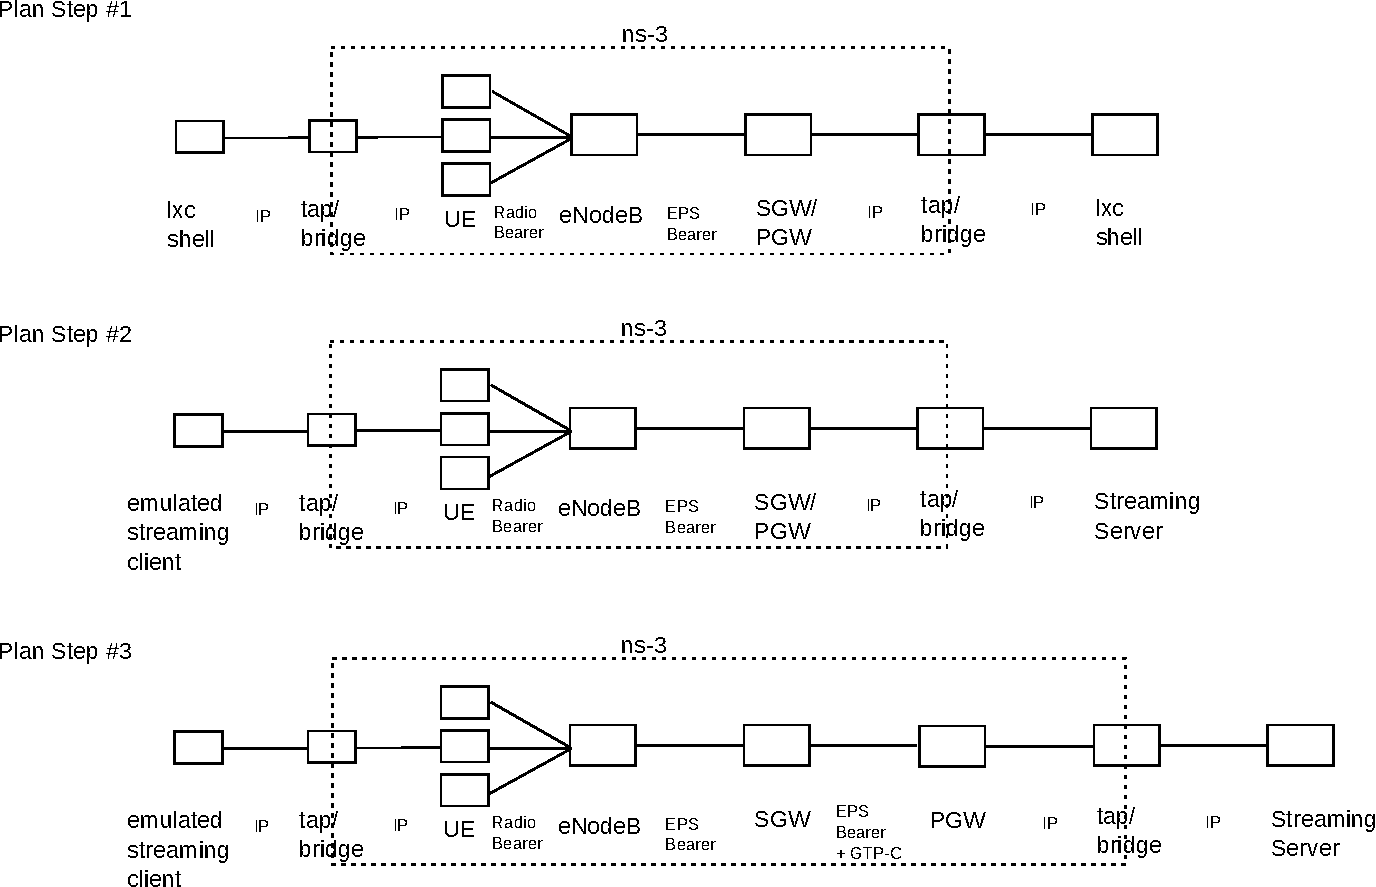
\includegraphics[width=\textwidth]{images/lte-testbed.pdf}
\caption{LTE Streaming Evaluation Setup and Action Plan}
\label{fig:lte-testbed}
\end{figure}